\documentclass{article}

\usepackage[utf8]{inputenc}
\usepackage[T1]{fontenc}
\usepackage[english]{babel}

\usepackage{graphicx}
\usepackage{courier}
\usepackage{charter}
\usepackage{xspace}

\usepackage{xcolor}
%\definecolor{butter}{HTML}{FCE94F}
%\definecolor{butter}{HTML}{EDD400}
\definecolor{butter}{HTML}{C4A000}
%\definecolor{orange}{HTML}{FCAF3E}
%\definecolor{orange}{HTML}{F57900}
\definecolor{orange}{HTML}{CE5C00}
%\definecolor{chocolate}{HTML}{E9B96E}
%\definecolor{chocolate}{HTML}{C17D11}
\definecolor{chocolate}{HTML}{8F5902}
%\definecolor{chameleon}{HTML}{8AE234}
%\definecolor{chameleon}{HTML}{73D216}
\definecolor{chameleon}{HTML}{4E9A06}
%\definecolor{skyblue}{HTML}{729FCF}
%\definecolor{skyblue}{HTML}{3465A4}
\definecolor{skyblue}{HTML}{204A87}
%\definecolor{plum}{HTML}{AD7FA8}
%\definecolor{plum}{HTML}{75507B}
\definecolor{plum}{HTML}{5C3566}
%\definecolor{scarletred}{HTML}{EF2929}
%\definecolor{scarletred}{HTML}{CC0000}
\definecolor{scarletred}{HTML}{A40000}
%\definecolor{lightalu}{HTML}{EEEEEC}
%\definecolor{lightalu}{HTML}{D3D7CF}
\definecolor{lightalu}{HTML}{BABDB6}
%\definecolor{darkalu}{HTML}{888A85}
%\definecolor{darkalu}{HTML}{555753}
\definecolor{darkalu}{HTML}{2E3436}

\newcommand{\kwstyle}{}

\usepackage{listings}

\lstset{
%	backgroundcolor=\color{},
	basicstyle=\small\ttfamily\color{black},
%	breakatwhitespace=false,
	breaklines=true,
%	captionpos=b,
	commentstyle=\color{darkalu},
%	deletekeywords={...},
%	escapeinside={\%*}{*)},
%	extendedchars=true,
%	frame=single,
%	keepspaces=true,
	keywordstyle=\kwstyle,
	language=Caml,
%	morekeywords={*,...},
%	numbers=left,
%	numbersep=5pt,
%	numberstyle=\color{},
%	rulecolor=\color{},
%	showspaces=false,
%	showstringspaces=false,
%	showtabs=false,
%	stepnumber=2,
	stringstyle=\color{plum},
	tabsize=2,
%	title=\lstname,
	keywordstyle=[1]\kwstyle\color{chameleon},
	keywordstyle=[2]\kwstyle\color{scarletred},
	keywordstyle=[3]\kwstyle\color{skyblue},
	keywordstyle=[4]\kwstyle\color{butter},
	keywordstyle=[5]\kwstyle\color{skyblue},
	keywordstyle=[6]\kwstyle\color{skyblue},
	keywordstyle=[7]\kwstyle\color{chameleon},
	keywordstyle=[8]\kwstyle\color{butter},
	keywordstyle=[9]\kwstyle\color{butter},
	keywords=[1]{let,val,method,in,and,rec,private,virtual,constraint},
	keywords=[2]{type,open,class,module,exception,external},
	keywords=[3]{fun,function,functor,match,try,with},
	keywords=[4]{as,when,of},
	keywords=[5]{if,then,else},
	keywords=[6]{begin,end,object,struct,sig,for,while,do,done,to,downto},
	keywords=[7]{true,false},
	keywords=[8]{include,inherit,initializer},
	keywords=[9]{new,ref,mutable,lazy,assert,raise},
}

\lstset{literate=
	{0}{{{\kwstyle\color{plum}0}}}1 {0.}{{{\kwstyle\color{plum}0.}}}2
	{1}{{{\kwstyle\color{plum}1}}}1 {1.}{{{\kwstyle\color{plum}1.}}}2
	{2}{{{\kwstyle\color{plum}2}}}1 {2.}{{{\kwstyle\color{plum}2.}}}2
	{3}{{{\kwstyle\color{plum}3}}}1 {3.}{{{\kwstyle\color{plum}3.}}}2
	{4}{{{\kwstyle\color{plum}4}}}1 {4.}{{{\kwstyle\color{plum}4.}}}2
	{5}{{{\kwstyle\color{plum}5}}}1 {5.}{{{\kwstyle\color{plum}5.}}}2
	{6}{{{\kwstyle\color{plum}6}}}1 {6.}{{{\kwstyle\color{plum}6.}}}2
	{7}{{{\kwstyle\color{plum}7}}}1 {7.}{{{\kwstyle\color{plum}7.}}}2
	{8}{{{\kwstyle\color{plum}8}}}1 {8.}{{{\kwstyle\color{plum}8.}}}2
	{9}{{{\kwstyle\color{plum}9}}}1 {9.}{{{\kwstyle\color{plum}9.}}}2
	{->}{{{\kwstyle\color{chameleon}$\rightarrow$}}}2
}


\usepackage{placeins}

\usepackage[colorlinks=true, citecolor=black, linkcolor=black, urlcolor=blue]{hyperref}

\usepackage{enumitem}
\setlist{itemsep=0mm}

\usepackage{colortbl}

\title{Weak models of data consistency}
\author{Benjamin Farinier}
\date{19/05/2014 -- 15/08/2014}

\newcommand{\irmin}{Irmin\xspace}
\newcommand{\git}{Git\xspace}
\newcommand{\lwt}{Lwt\xspace}
\newcommand{\mercurial}{Mercurial\xspace}
\newcommand{\mirage}{Mirage\xspace}
\newcommand{\obj}{Obj\xspace}
\newcommand{\ocaml}{OCaml\xspace}
\newcommand{\opam}{OPAM\xspace}
\newcommand{\xen}{Xen\xspace}

\newcommand{\code}[1]{\texttt{#1}}

\begin{document}

\maketitle
\tableofcontents

\section[\mirage, an \ocaml-based unikernel system]{\mirage, an \ocaml-based unikernel system\\\normalsize\normalfont(based on the \href{http://openmirage.org}{\texttt{openmirage.org}} website)}

\begin{figure}[hbt]
\centering
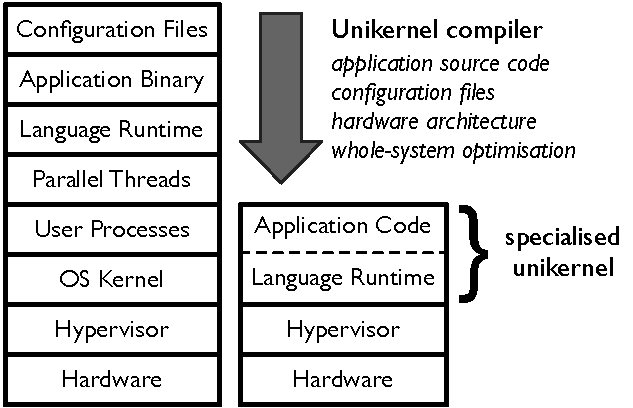
\includegraphics[scale=0.8]{images/mirage-stack.pdf}
\caption{Contrasting software layers in existing VM appliances vs. unikernel’s standalone kernel compilation approach.}
\label{miragestackgraph}
\end{figure}

Because they rely on an underlying operating system, most applications that run in the cloud aren't optimised to do so.
Compartmentalisation of large servers into smaller virtual machines has enabled many new businesses to get started and achieve scale.
But many of those virtual machines are single-purpose and yet they contain largely complete operating systems, including their vulnerabilities and bloat.
\mirage represents a new approach where only the necessary components of the OS are included and compiled along with the application into a unikernel.
This results in highly efficient appliances that can be deployed directly to the cloud and embedded devices, with the benefits of reduced costs and increased security and scalability. The figure~\ref{miragestackgraph} describes the difference between unikernels and current approaches.

\mirage is a \emph{library operating system}\cite{LibraryOperatingSystemsCloud2013} designed for constructing secure, high-performance network applications across a variety of cloud computing and mobile platforms.
It is based around the \xen hypervisor and the \ocaml langage.
\xen provides a stable hardware platform\cite{XenArtVirtualization2003}, which avoids the need to support the thousands of device drivers found in a traditional OS.
Thanks to \ocaml, code can be developed in a high-level functional programming language which avoids many of usual flaws\cite{CreatingFunctionalInternet2007}.
It is then compiled into a fully-standalone, specialised unikernel which can run directly on \xen hypervisor APIs.
Since \xen powers most public clouds, \mirage lets you deploy your servers more cheaply, securely and faster in any of them.

Due to the much smaller size, it is possible for example to create auto-scaling web-servers with very small footprints.
If a sudden spike in traffic occurs, the web-servers can be configured to create and deploy copies of themselves to serve the demand.
This auto-scaling can happen so quickly that an incoming connection can trigger the creation of new server and the new server can then handle that request before it times out (which is on the order of milliseconds).
When the demand dies down again, these web-servers can automatically shut themselves down.
This elasticity results in the ability to precisely match the demand and avoid wasting resources.

\paragraph{Towards a distributed database}
As a cloud oriented operating system, \mirage has to deal with all the problems arising in distributed systems.
One of them is to share data between several devices spread out over a network.
In the example of self-scaling web-servers, newly created instances should first fork an image of the web-server's global current state.
Then they can modify it independently according to the requests they receive.
Finally, when the traffic is decreasing and returning to a normal rate, the forked web-servers have to somehow merge back all their local modifications.
Understanding how to merge them efficiently is the purpose of my internship.



\section{\irmin, a large-scale, immutable, branch-consistent storage}

\subsection{Design}

\irmin is a portable distributed database written in \ocaml, and designed with the requirements of static type-safety for security and reliability.
Designing a distributed database is a difficult problem, mainly because of the CAP theorem\cite{BrewerConjecture2002} which states that:

\bigskip
\begin{tabular}{|c}
\begin{minipage}{0.9\textwidth}
It is impossible for a distributed system to simultaneously provide all three of the following guarantees:
\begin{enumerate}
	\item \emph{Consistency}: all nodes see the same data at the same time
	\item \emph{Availability}: a guarantee that every request receives a response about whether it was successful or failed
	\item \emph{Partition tolerance}: the system continues to operate despite arbitrary message loss or failure of part of the system.
\end{enumerate}
\end{minipage}
\end{tabular}
\bigskip

The modern answer to solve this paradox is to maintain availability but relax the consistency model.
Most of the large-scale distributed systems assume there is no unique global state of the system, which results in a class of system said to be \emph{eventually consistent}\cite{EventuallyConsistentTransactions2012}.
The approach of \irmin to relax the consistency model is inspired by distributed version control systems such as \git and \mercurial.
Every actor owns a branch representing a partial replica of the global database.
Modifications are local and happen only on the current branch.
Branches can explicitly be merged in order to recover the consistency property, using application-defined merge policies between replicas.
Such classes of systems have been called \emph{branch-consistent} models.

Data replication is a key technology in distributed systems that enables higher availability and performance.
It is possible to distinguish two kinds of replication:
\emph{pessimistic}\cite{ImplementingFaulttolerantServices1990}\cite{ParttimeParliament1998}\cite{UnderstandableConsensusAlgorithm2014} methods where master election and synchronous locking are used to block the system while changes are propagated;
and \emph{optimistic}\cite{OptimisticReplication2005} methods where the changes are propagated in the background and where special techniques handle supposed rare conflicts.
\irmin chooses to use an optimistic replication system because it improves availability, does not need knowledge about the underlying network, and can easily scale because it does not need synchronisation.
The drawback is that the users have to handle conflicts.

Conflicts can appear in two different situations:
when two nearby users are modifying the same value at the same time;
and when a value has been changed in two distant locations, with the background propagation resulting in a conflict.
\irmin allows the application developer to deal with these situations using several tools:
\begin{itemize}
	\item Conflict-free replicated data types\cite{ConflictfreeReplicatedDataTypes2011}
	\item Type of data with custom merge operator
	\item Callback functions applied every time a conflict happen
\end{itemize}
The study and the design of such mechanisms is one of the main goals of my internship.


\subsection{Architecture}

\begin{figure}[hbt]
\begin{lstlisting}
module type S = sig
  type t
  type path
  type contents

  val read: t -> path -> contents
  (** Read the content at [path] in [t]. *)
  val update: t -> path -> contents -> unit
  (** Replace the contents at [path] in [t] by [contents] if [path] is already defined and create it otherwise. *)
  val remove: t -> path -> unit
  (** Remove the given [path] in [t]. *)
  ...
end
\end{lstlisting}
\caption{High-level prefix-tree interface of \irmin, generated over the block store, the tag store and the application contents description.}
\label{prefixtreesig}
\end{figure}

\irmin provides a high-level interface built upon two user-provided stores.

The \emph{block store} is a low-level key/value append-only store, where values are a sequence of bytes and keys are deterministically computed from the values (for instance using SHA algorithms).
This mean that:
\begin{itemize}
	\item if a value is modified, a new key/value pair is created: the resulting data-store is \emph{immutable}
	\item if two data-stores share the same values, they will have the same keys: the store is \emph{consistent}, the overall structure only depend on the stored data
\end{itemize}
The block store contains serialized values from application contents, but also structured data, like prefix-tree nodes and history meta-data.
As the store is append-only, there is no remove function.
The store is expected to grow forever, but garbage-collection and compression techniques can be used to manage its growth.
This is not an issue as commodity storage steadily becomes more and more inexpensive.

The tag store is the only mutable part of the system.
It is a key/value store, where keys are names created by users and values are keys from the block store, and can be seen as a set of named pointers to keys in the block store.
This store is expected to be local to each replica and very small.
The tag store is central for higher-level algorithms such as synchronisation and garbage collection.

The high-level interface is generated over the block store, the tag store and the application contents description.
It lifts immutable operations on the block store into a mutable prefix-tree, whose signature is given in figure~\ref{prefixtreesig}.
The prefix tree \code{path} is usually a list of strings and node values are the user-defined mergeable \code{contents}.
The complete signature of such contents is detailed in appendix~\ref{appendixcontent}.



\section{Weakly consistent data structures}

As mentioned earlier, \irmin allows the application developer to deal with conflicts using several tools.
One of them is the use of data structures with custom merge operators.
The idea is to give an abstraction of the \irmin low-level store as a high-level data structure.
In addition of their classical operations, these data structure include the merge operation mentioned earlier. 
In this paper, we will considered queue and rope data structures.

These data structures and their associated operations have already been widely studied, even in a pure functional context\cite{PurelyFunctionalDataStructures1996}.
\textbf{That is why the purpose of this work is not to compete with existing implementations of such data structures, but to extend them with an efficient and consistent merge operation.}



\subsection{Queues}

There are several efficient implementations of queues that can perform enqueuing (or \emph{push}) and dequeuing (or \emph{pop}) operations in $O(1)$ time.
However, \irmin is built on an append-only low-level store.
Such representations of the memory matches well with the functional programming model where the memory is immutable.
For this reason I design these mergeable queues as functional queues.
The exposed signature is presented in appendix~\ref{appendixqueue}.

\begin{figure}[hbt]
\centering
\setlength{\tabcolsep}{0.5cm}
\begin{tabular}{|c|c|c|c|}
\hline
	Operation &
	Read &
	Write &
	\\
\hline
	Push &
	\cellcolor{chameleon!20} $0$ &
	\cellcolor{chameleon!20} $2$ &
	\cellcolor{chameleon!20} $O(1)$ \\
\hline
	Pop &
	\cellcolor{butter!20} $2$ on average &
	\cellcolor{butter!20} $1$ on average &
	\cellcolor{chameleon!20} $O(1)$ \\
\hline
\hline
	Merge &
	\cellcolor{scarletred!20} $n$ worst case &
	\cellcolor{chameleon!20} $1$ &
	\cellcolor{butter!20} $O(n)$ \\
\hline
\end{tabular}
\caption{Cost of queue operations where $n$ denotes the length of the queue. Read and write are expressed in number of memory access.}
\label{queuetable}
\end{figure}

A functional queue is composed of two simple linked lists.
The first one contains elements that have been pushed onto the queue, and the second one those that will be popped.
When the pop list is empty, the push list is flushed into the pop one.
This operation is called \emph{normalization}.
Event though the normalization is a linear operation,  each element of the queue has to be normalized only once.
That is why --as it is reminded in figure~\ref{queuetable}-- the amortized cost of operations on the queue is $O(1)$.

\paragraph{Internal structure}
The implementation of mergeable queues is based on an \irmin store containing three types of element: \code{Index}, \code{Node} and \code{Elt}. Their type declarations are given in figure~\ref{queuesig}.

\code{Index} are queue accessors.
They are defined by four fields, \code{push}, \code{pop}, \code{top} and \code{bottom}.
The two first fields, \code{push} and \code{pop}, are the number of pushes and pops applied to the queue since its creation.
They are useful for the merge operation.
The two others, \code{top} and \code{bottom}, are keys of the top and bottom element of the queue.

\code{Node} are elements manipulated by queue operations.
They are composed of four optional elements, \code{next}, \code{previous}, \code{elt} and \code{branch}. \code{next} and \code{previous} are keys to a potential preceding or following element.In practice, only one of these two can be not empty. \code{elt} is also an optional key which points to a value of the queue. The last field \code{branch} is an optional index, used only by the merge operation.

Finally, \code{Elt} contains elements added to the queue.

\begin{figure}[hbt]
%\begin{lstlisting}
%type index = {              type node = {
%  push: int;                  next: K.t option;
%  pop: int;                   previous: K.t option;
%  top: K.t;                   elt: K.t option;
%  bottom: K.t;                branch: index option;
%} with compare, sexp        } with compare, sexp
%
%type elt = Index of index | Node of node | Elt of V.t
%           with compare, sexp
%\end{lstlisting}
\begin{lstlisting}
type index = {              type node = {
  push: int;                  next: K.t option;
  pop: int;                   previous: K.t option;
  top: K.t;                   elt: K.t option;
  bottom: K.t;                branch: index option;
}                           }

type elt = Index of index | Node of node | Elt of V.t
\end{lstlisting}
\caption{Type declaration of mergeable queue structuring elements. The \irmin store is specialized in order to containing such elements.}
\label{queuesig}
\end{figure}

\paragraph{Major operation}
The two first main operations on a queue are push and pop.
The push operation adds a new \code{Elt} containing the pushed value, and a \code{Node} pointing to this element and the previous bottom element of the queue.
It returns a new \code{Index} where the bottom element is the new created \code{Node}.
The pop operation tries to read the top element of the queue.
If the pop list is empty, the queue is normalized.
Then it returns the value associated with the reading \code{Node} and an \code{Index}, where the top element is the following element of the reading \code{Node}.
On average, there are two reads and three writes in the \irmin store for one push and one pop.

The other main operation is merging.
The merging operation takes three arguments: two queues to be merged, \code{q1} and \code{q2}, and a common ancestor to those two queues called \code{old}.
The resulting queue -- called \code{new} -- has to reflect the transformations from \code{old} to both \code{q1} and \code{q2}.
First, elements of \code{old} which have been removed from \code{q2} are removed from \code{q1}.
This is done without accessing these elements by using the \code{push} and \code{pop} values.
In the same way, all elements of \code{old} which are still in \code{q2} are removed.
Then, \code{q2} is concatenated at the end of \code{q1} by adding a new node where the field \code{branch} contains the index of \code{q2}.
In the worst case, the merge operation uses a number of reads linear in the size of \code{old}, but always only one write.

\begin{figure}[hbt]
\centering
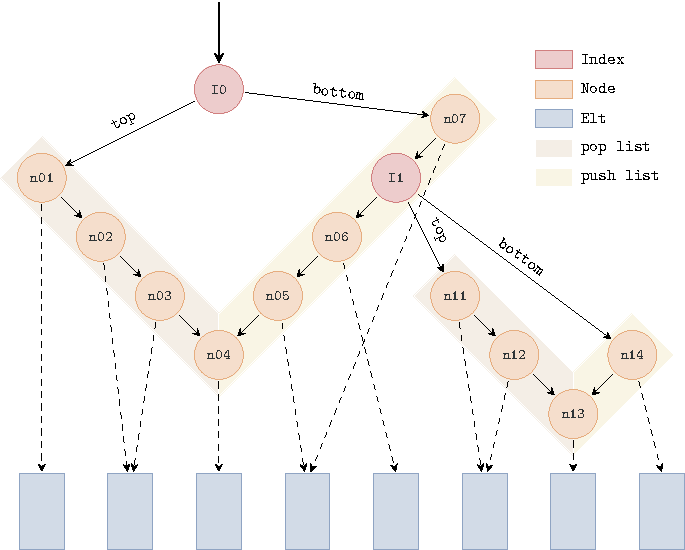
\includegraphics[scale=0.8]{images/queue.pdf}
\caption{Example of a possible queue internal structure. Here, the main queue is accessible through the index \code{I0}. The index \code{I1} is pointing to a queue concatenated during a previous merge operation. This queue will be unfolded during the next normalization. Because of the \irmin store behavior,  two nodes containing the same element share its physical representation.}
\label{queuegraph}
\end{figure}


\subsection{Ropes}

\paragraph{General description}
A rope is a data structure that is used for efficiently storing and manipulating a very long string.
A rope is a binary tree having leaf nodes that contain a short string.
Each node has an index equal to the sum of the length of each string in its left subtree.
Thus a node with two children divides the whole string into two parts: the left subtree stores the first part of the string and the right subtree stores the second part.
The binary tree is crossed from the root to leaf each time the string has to be accessed.
It can be done in $\log (n)$ time if the tree is balanced.

The main operations on a rope are \emph{set}, \emph{get}, \emph{split}, \emph{concatenate}, \emph{insert} and \emph{delete}:
Set and get respectively set or get the character at a given position.
Split$(t, i)$ split at the position $i$ the rope $t$ into two new rope.
Concatenate$(t_1, t_2)$ return a new rope which is the concatenation of $t_1$ and $t_2$.
Insert$(t, i, s)$ insert the character chain $s$ in the rope $t$ at the position $i$.
Finally, Delete$(t, i, j)$ delete in the rope $t$ the characters between $i$ and $j$.
Figure~\ref{ropetable} compares the complexity of these operations for a rope and a string.

If ropes are mainly used to manipulate strings, they can also be used to manipulate any other type of container, as long as they support the above six operations.
In fact, I design the ropes with the following idea:
"give me a container with a set of operations, and I will return you a rope on this container, supporting the same operations but achieving a better complexity, with the exception of set and get".
I therefore request a merge operation on the container in order to implement the merge operation of the mergeable rope.
Indeed, because such a rope can be built on any type of container, it is impossible to have a general way to merge it.

\begin{figure}[hbt]
\centering
\setlength{\tabcolsep}{1cm}
\begin{tabular}{|c|c|c|}
\hline
	Operation &
	Rope &
	String \\
\hline
	Set/Get &
	\cellcolor{butter!20} $O(\log n)$ &
	\cellcolor{chameleon!20} $O(1)$ \\
\hline
	Split &
	\cellcolor{butter!20} $O(\log n)$ &
	\cellcolor{chameleon!20} $O(1)$ \\
\hline
	Concatenate &
	\cellcolor{butter!20} $O(\log n)$ &
	\cellcolor{scarletred!20} $O(n)$ \\
\hline
	Insert &
	\cellcolor{butter!20} $O(\log n)$ &
	\cellcolor{scarletred!20} $O(n)$ \\
\hline
	Delete &
	\cellcolor{butter!20} $O(\log n)$ &
	\cellcolor{scarletred!20} $O(n)$ \\
\hline
\hline
	Merge &
	\cellcolor{chameleon!20} $\log\left(f(n)\right)$ &
	\cellcolor{butter!20} $f(n)$ \\
\hline
\end{tabular}
\caption{Comparison of the complexity of several operations on ropes and strings. $n$ denotes the length of the rope/string, and $f$ is the complexity of the merge function provided by the user.}
\label{ropetable}
\end{figure}

%\begin{figure}[hbt]
%\centering
%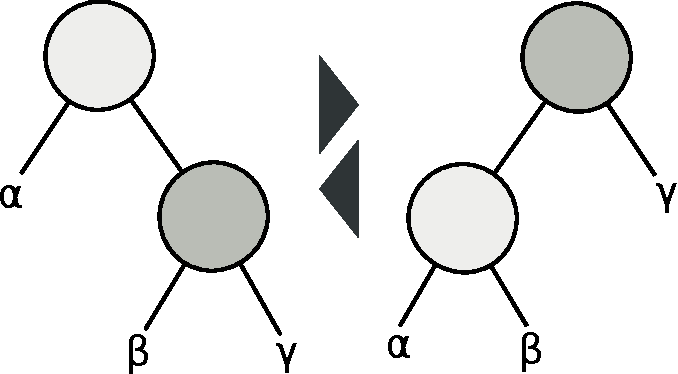
\includegraphics[scale=0.6]{rotations.pdf}
%\caption{Generic tree rotation. A tree rotation moves one node up in the tree and one node down.}
%\label{rotationgraph}
%\end{figure}

\paragraph{Implementation overview}
The implementation of mergeable ropes is quite straightforward, in the sense that it follows the previous description, and its signature is given in appendix~\ref{appendixrope}.
The tree containing the rope is a self-balancing binary search tree which keeps a factor of two between its minimal and maximal depth.
To implement such tree, the \irmin store is specialized in order to contain three types of elements.
As in mergeable queue, \code{Index} are accessors to the data structure.
\code{Node} are intermediate elements of the tree which contain information to improve the binary search.
Finally, \code{Leaf} are the user-defined container on which the rope is built.

The implementations of the six main operations follow more or less the same pattern.
The algorithm performs a binary search on the tree in order to determine the leaves concerned by the operation.
Then the operation is applied on the containers found in the leaves.
In order to achieve the $\log n$ complexity, the size of these containers has to be of the same order as the depth of the tree.
Finally, the tree is recursively rebuilt, using a rotation transformation in order to maintain the balancing property.

The merge operation is a bit different.
Given two trees to be merged and their common ancestor, their keys in the \irmin store are used to determine the smallest subtrees where modifications occurred.
Then these subtrees are linearised in containers on which the user-defined merge operation is applied.
On simple trees, this approach is very efficient because the merge operation is applied on the smallest possible container.
However, the balancing property reduces this effectiveness.
Indeed, the internal structure of a tree can be deeply modified during a rebalancing operation, making it impossible to compare potentially large subtrees.
In order to minimize the scope of rebalancing operations, the rotation function is applied as little as possible, and only on the smallest unbalanced subtree.
Due to this restriction, the impact on the merge function efficiency is proportional to the volume of modifications produced by  an operation.


\section{Data structure analysis}

After having implemented those two data structures, it was necessary to assert the correctness of these implementations and to analyse their effective costs.

\subsection{Automatic checking}

In the case of the correctness, we especially want to ensure that the classical operations match with their equivalents in other implementations, and that the merge operation follows its specification.
The way it works is similar for queues and ropes.
An oracle is used to determine a sequence of operations and their result.
This sequence is then applied on the tested data structure, and on a witness obtained from another implementation.
At each step, the data structure and the witness are required to exactly match.
And at the end of the sequence, the two obtained result have to correspond with the result predicted by the oracle.

If this protocol is working fine with classical operations, it cannot be honestly applied on the merge operation.
Indeed, it does not exist at my knowledge another data structure to be used as a witness.
The verification process is therefore a bit different for this operation.
In this case, we chose a result with a easily verifiable property which is preserved after each merge operation.
For example, a queue containing an increasing sequence of numbers, or a rope composed by a nondecreasing sequence of characters.
This result is decomposed in several subresult having to be merge in order to recover the initial one.
And because a merge preserves the aforementioned property, we can verify the correctness of the merge operation at each of its uses.

These tests have successfully guaranteed the good behaviors of my implementation of queues and ropes data structures.
But they are not sufficient to ensure that the theoretical complexity is reached.
In addition, I therefore designed several benchmark tests in order to validate this last point.
Aside from showing the theoretical complexity is reached, these tests highlight some other interesting facts.


\subsection{Benchmarking}

\paragraph{Performance analysis}
The most obvious interest of benchmark tests is to measure the needed time of a given operation.
The figure~\ref{ropeduration} shows the result of one of these tests.
As a first glance, we can see that the theoretical complexity is reached for every operations.
Then we can see a general stair behaviors.
This one is due to the internal tree representation.
Indeed, at each a step a new level is needed in this tree in order to represent the whole rope.
Finally, we can see several spikes, which are the consequences of the complex interactions between the balancing property and maintaining a leaf length proportional to the depth of the tree.

\begin{figure}[hbt]
\centering
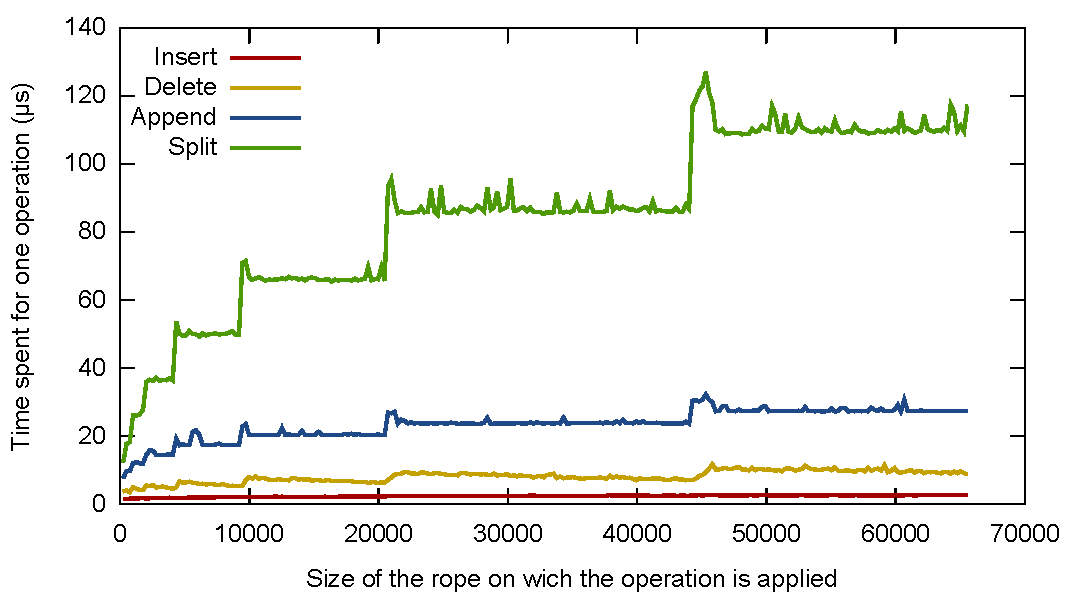
\includegraphics[scale=0.6]{images/rope_duration.pdf}
\caption{Needed time for one operation on a rope of size $n$ on the \obj backend~(see later)}
\label{ropeduration}
\end{figure}

\paragraph{Backend comparison}
As \irmin can be instantiated on different backends, it may be interesting to compare their relative performances.
The figure~\ref{queuebackend} shows the result of a same test run on different backends.
On this graph, \emph{Memory} refers to the in RAM backend.
\emph{GitMem} and \emph{GitDsk} respectively refer to a \git backend, in the first case instantiate in the memory, on the hard drive in the second case.

The two last are a slightly different.
\emph{\obj} is backend based on the \ocaml module \obj that I have implemented.
The idea is to directly manipulate the \ocaml heap.
In a sense, that gives the raw cost of the algorithm.
Its implementation is given in appendix~\ref{appendixobj}.
Finally \emph{Core} is not strictly a backend because it refers in fact to the implementation of functional queue in the Core library.
It is used here as a sort of optimal case, in a matter of comparison.

As we can see, there is a factor five between Core and the implementation of my queue on the \obj backend.
It is an acceptable price to pay for maintaining a mergeable data structure.

\begin{figure}[hbt]
\centering
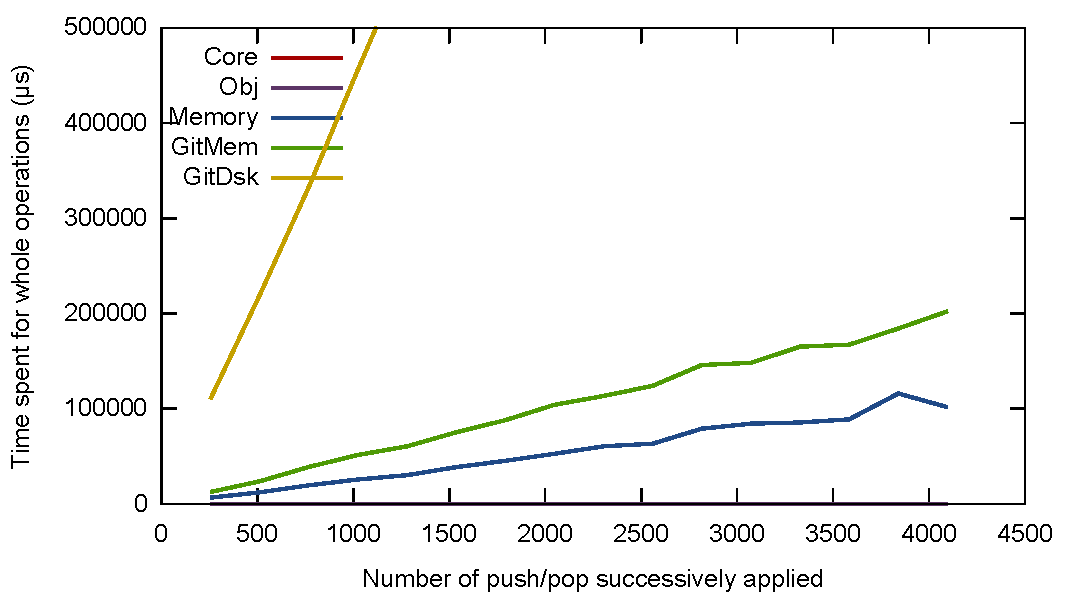
\includegraphics[scale=0.6]{images/queue_backend.pdf}
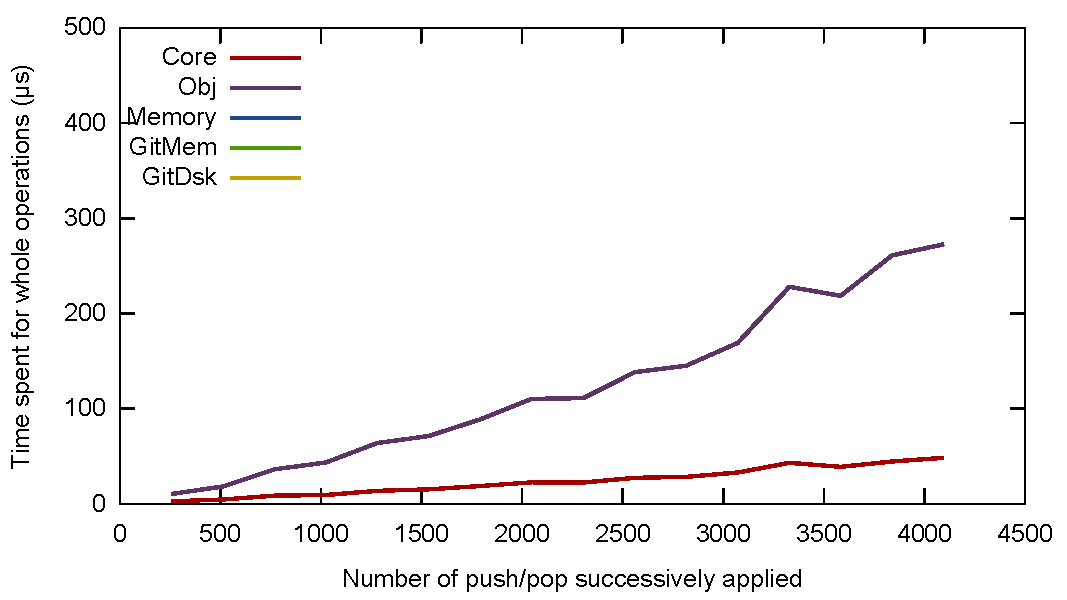
\includegraphics[scale=0.6]{images/queue_zoom.pdf}
\caption{Time needed for $n$ push followed by $n$ pop on different backends}
\label{queuebackend}
\end{figure}

\paragraph{IO cost estimation}
A last original use of benchmarks is the possibility to determine the time needed for a read and a write on different backends.
Indeed, my rope implementation is able to produce some statistics about the number of read and write used in each operation.
Some results of this statistics are given in the figure~\ref{ropereadwrite}.

Aside from highlighting the obvious fact that the cost of an operation is proportional to the number of read and write, we can see that the relative proportion of read and write is different in each operation.
Knowing the time needed for one operation, these proportions give us a linear system of four independent equation where variables are the time needed for a read and a write, represented in figure~\ref{interpolation}.
The average of intersection points indicates the solution that we looking for.

\begin{figure}[hbt]
\centering
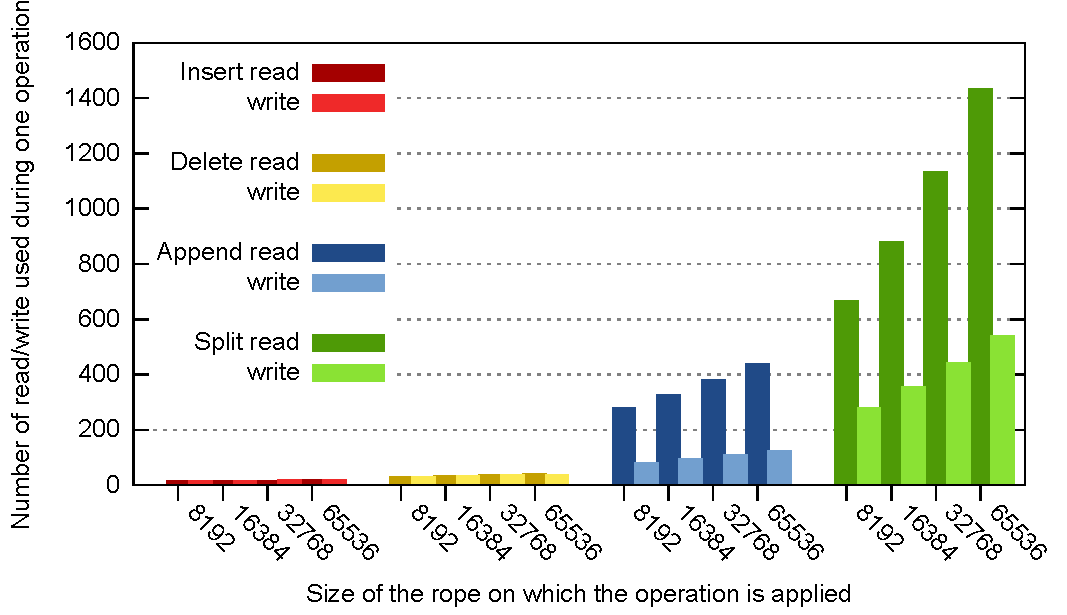
\includegraphics[scale=0.6]{images/rope_readwrite.pdf}
\caption{Number of read/write used during one operation on a rope of size $n$.}
\label{ropereadwrite}
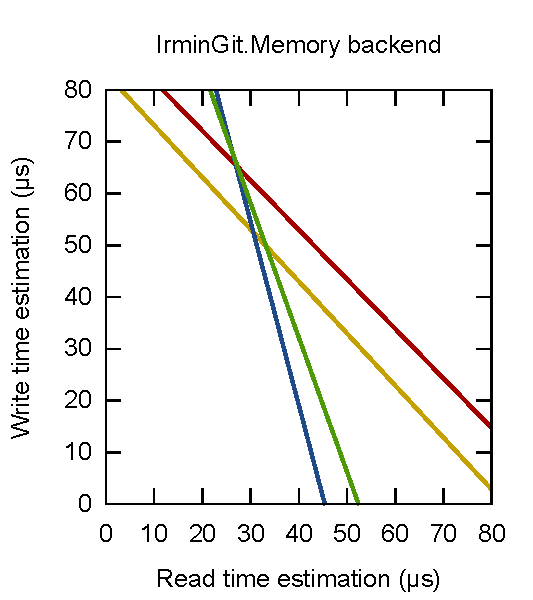
\includegraphics[scale=0.6]{images/git_interp.pdf}
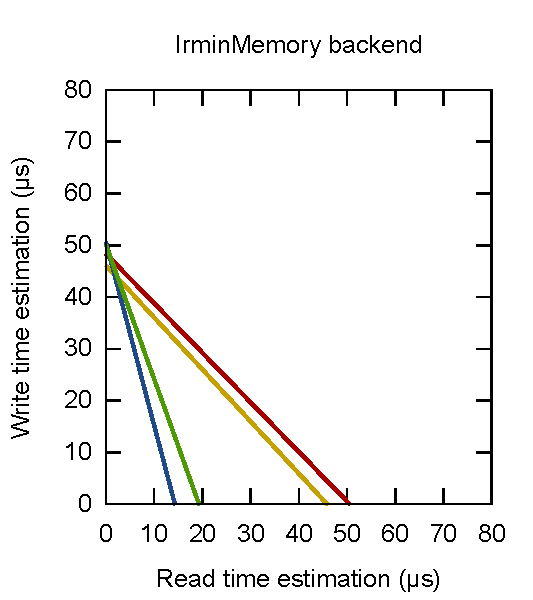
\includegraphics[scale=0.6]{images/mem_interp.pdf}
\caption{Let $x$ be the time needed for one read, $y$ the time needed for one write and $d$ the time needed for one operation on a rope. Then the above curves --where colors match with the previous figure-- are the plot of the equation: $x * \mbox{nrb of read} + y * \mbox{nbr of write} = d$}
\label{interpolation}
\end{figure}

\section{Conclusion and future works}

At the end of my internship, I have implemented mergeable queues and ropes, and an \irmin \obj backend.
I have also run several benchmark tests which provided several useful result.

In the future, I plan to keep collaborating with the \mirage team by maintaining and improving the libraries I have released during my internship.
For instance, I would like to improve the implementation of the mergeable queues, in order to reach a $\log(n)$ complexity for the merge operation.
I would also like to work on the use GADTs in order to reduce the cost of several operations.

During my internship, I have also designed a very first draft of a mergeable priority heap, that I would like to try to properly implement and release.
Finally, produce some concrete use case of my data structure could be a long-term project.

\FloatBarrier

\nocite{*}
\bibliographystyle{plain}
\bibliography{biblio.bib}

\newpage

\section*{Appendix}
\addtocounter{section}{1}
\setcounter{subsection}{0}
\addcontentsline{toc}{section}{Appendix}
\renewcommand{\thesubsection}{\Alph{subsection}}

\subsection{\irmin content signature\label{appendixcontent}}
\begin{lstlisting}
module type S = sig
(** Signature for store contents. *)

  include IrminIdent.S
  (** Base types. *)

  val merge: t IrminMerge.t
  (** Merge function. Raise [Conflict] if the values cannot be merged properly. *)

end

module type STORE = sig
(** Signature for store contents. *)

  include IrminStore.AO
  (** Contents stores are append-only. *)

  val merge: t -> key IrminMerge.t
  (** Store merge function. Lift [S.merge] to keys. *)

  module Key: IrminKey.S with type t = key
  (** Base functions for foreign keys. *)

  module Value: S with type t = value
  (** Base functions for values. *)

end

module Make
    (K: IrminKey.S)
    (C: S)
    (Contents: IrminStore.AO with type key = K.t and type value = C.t)
  : STORE with type t = Contents.t
           and type key = K.t
           and type value = C.t
(** Build a contents store. *)

module Rec (S: STORE): S with type t = S.key
(** Convert a contents store objects into storable keys, with the expected merge function (eg. read the contents, merge them and write back the result to get the final key). *)
\end{lstlisting}

\bigskip


\subsection{Mergeable queue signature\label{appendixqueue}}
\begin{lstlisting}
module type S = sig

  include IrminContents.S
  (** The type of queues. *)

  type elt
  (** The elements of the queues. *)

  val create : unit -> t Lwt.t
  (** Create a new queue. *)

  val length : t -> int Lwt.t
  (** Return the length of the queue [t]. *)

  val is_empty : t -> bool Lwt.t
  (** Return true if the given queue [t] is empty, false otherwise. *)

  val push : t -> elt -> t Lwt.t
  (** Returns a queue with adds [value] to the end of [t]. Complexity: O(1). *)

  val pop : t -> (elt * t) Lwt.t
  (** Returns the top element and a version of the queue where it is removed. Raise [Empty] if the queue is empty. Complexity: amortized O(1). *)

  val peek : t -> (elt * t) Lwt.t
  (** Returns the top element and a version of the queue updated but inchanged. Raises [Empty] if no element is found. Complexity: O(1). *)

  val dump : t -> string Lwt.t
  (** Dump the contents of the queue. *)

end

module Make
    (AO: Irmin.AO_MAKER)
    (K: IrminKey.S)
    (V: IrminIdent.S)
  : S with type elt = V.t
\end{lstlisting}

\bigskip


\subsection{Mergeable rope signature\label{appendixrope}}
\begin{lstlisting}
module type S = sig

  include IrminContents.S    (** The type of ropes *)
  type value                 (** e.g char *)
  type cont                  (** e.g string *)


  val create : unit -> t Lwt.t
  (** Create a new empty rope. *)
  val make : cont -> t Lwt.t
  (** Construct a new rope from the container [cont] *)
  val flush : t -> cont Lwt.t
  (** Return the container represented by the rope [t] *)


  val is_empty : t -> bool Lwt.t
  (** Return true if the rope [t] is empty, false otherwise. *)
  val length : t -> int Lwt.t
  (** Return the length of the rope [t]. *)


  val set : t -> pos:int -> value -> t Lwt.t
  (** Set the value at the position [pos] in the rope [t] to [value]. Complexity: log(n) *)
  val get : t -> pos:int -> value Lwt.t
  (** Get the value containing in the rope [t] at the position [pos]. Complexity: log(n) *)
  val insert : t -> pos:int -> cont -> t Lwt.t
  (** Insert the container [cont] in the rope [t] at the position [pos]. Complexity: log(n) *)
  val delete : t -> pos:int -> len:int -> t Lwt.t
  (** Delete [len] elements after the position [pos] in the rope [t]. Complexity: log(n) *)
  val append : t -> t -> t Lwt.t
  (** Append the two given ropes. Complexity: log(n) *)
  val concat : sep:t -> t list -> t Lwt.t
  (** Concatenate the ropes containing in [list] with the separator [sep]. Complexity: Sum (log n) *)
  val split : t -> pos:int -> (t * t) Lwt.t
  (** Split the rope [t] at the position [pos] into two ropes. Complexity: log(n) *)

end
\end{lstlisting}

\bigskip

\begin{lstlisting}
module Make
    (AO: Irmin.AO_MAKER)
    (K: IrminKey.S)
    (V:
     sig
       type a
       type t
       include IrminIdent.S with type t := t

       val empty : t

       val length : t -> int
       val set : t -> int -> a -> t
       val get : t -> int -> a
       val insert : t -> int -> t -> t
       val delete : t -> int -> int -> t
       val append : t -> t -> t
       val concat : t -> t list -> t
       val split : t -> int -> (t * t)

       val merge : t IrminMerge.t
     end)
  : S with type value = V.a
       and type cont = V.t

\end{lstlisting}

\bigskip


\subsection{\obj backend implementation\label{appendixobj}}
\begin{lstlisting}
module ObjBackend
    (K: IrminKey.S)
    (V: IrminIdent.S) :
  (IrminStore.AO with type key = K.t
                  and type value = V.t) = struct

  type t = unit
  type key = K.t
  type value = V.t

  let create () = return ()
  let clear () = return ()

  let add t value =
    return (Obj.magic (Obj.repr value))

  let read t key =
    return (Some (Obj.obj (Obj.magic key)))

  let read_exn t key =
    return (Obj.obj (Obj.magic key))

  let mem t key = return true
  let list t k = return k
  let dump t = return []

end
\end{lstlisting}

\end{document}
